%%
%% This is file `sample-sigconf.tex',
%% generated with the docstrip utility.
%%
%% The original source files were:
%%
%% samples.dtx  (with options: `sigconf')
%% 
%% IMPORTANT NOTICE:
%% 
%% For the copyright see the source file.
%% 
%% Any modified versions of this file must be renamed
%% with new filenames distinct from sample-sigconf.tex.
%% 
%% For distribution of the original source see the terms
%% for copying and modification in the file samples.dtx.
%% 
%% This generated file may be distributed as long as the
%% original source files, as listed above, are part of the
%% same distribution. (The sources need not necessarily be
%% in the same archive or directory.)
%%
%%
%% Commands for TeXCount
%TC:macro \cite [option:text,text]
%TC:macro \citep [option:text,text]
%TC:macro \citet [option:text,text]
%TC:envir table 0 1
%TC:envir table* 0 1
%TC:envir tabular [ignore] word
%TC:envir displaymath 0 word
%TC:envir math 0 word
%TC:envir comment 0 0
%%
%%
%% The first command in your LaTeX source must be the \documentclass
%% command.
%%
%% For submission and review of your manuscript please change the
%% command to \documentclass[manuscript, screen, review]{acmart}.
%%
%% When submitting camera ready or to TAPS, please change the command
%% to \documentclass[sigconf]{acmart} or whichever template is required
%% for your publication.
%%
%%
\documentclass[sigconf]{acmart}
\usepackage{listings}
%%
%% \BibTeX command to typeset BibTeX logo in the docs
\AtBeginDocument{%
  \providecommand\BibTeX{{%
    Bib\TeX}}}

%% Rights management information.  This information is sent to you
%% when you complete the rights form.  These commands have SAMPLE
%% values in them; it is your responsibility as an author to replace
%% the commands and values with those provided to you when you
%% complete the rights form.
\setcopyright{acmcopyright}
\copyrightyear{2018}
\acmYear{2018}
\acmDOI{XXXXXXX.XXXXXXX}

%% These commands are for a PROCEEDINGS abstract or paper.
\acmConference[Conference acronym 'XX]{Make sure to enter the correct
  conference title from your rights confirmation emai}{June 03--05,
  2018}{Woodstock, NY}
%%
%%  Uncomment \acmBooktitle if the title of the proceedings is different
%%  from ``Proceedings of ...''!
%%
%%\acmBooktitle{Woodstock '18: ACM Symposium on Neural Gaze Detection,
%%  June 03--05, 2018, Woodstock, NY}
\acmPrice{15.00}
\acmISBN{978-1-4503-XXXX-X/18/06}


%%
%% Submission ID.
%% Use this when submitting an article to a sponsored event. You'll
%% receive a unique submission ID from the organizers
%% of the event, and this ID should be used as the parameter to this command.
%%\acmSubmissionID{123-A56-BU3}

%%
%% For managing citations, it is recommended to use bibliography
%% files in BibTeX format.
%%
%% You can then either use BibTeX with the ACM-Reference-Format style,
%% or BibLaTeX with the acmnumeric or acmauthoryear sytles, that include
%% support for advanced citation of software artefact from the
%% biblatex-software package, also separately available on CTAN.
%%
%% Look at the sample-*-biblatex.tex files for templates showcasing
%% the biblatex styles.
%%

%%
%% The majority of ACM publications use numbered citations and
%% references.  The command \citestyle{authoryear} switches to the
%% "author year" style.
%%
%% If you are preparing content for an event
%% sponsored by ACM SIGGRAPH, you must use the "author year" style of
%% citations and references.
%% Uncommenting
%% the next command will enable that style.
%%\citestyle{acmauthoryear}


%%
%% end of the preamble, start of the body of the document source.
\begin{document}

%%
%% The "title" command has an optional parameter,
%% allowing the author to define a "short title" to be used in page headers.
\title{CS 527 SP23 Course Project \\ FreeFuzz Extension for PaddlePaddle}
%%
%% The "author" command and its associated commands are used to define
%% the authors and their affiliations.
%% Of note is the shared affiliation of the first two authors, and the
%% "authornote" and "authornotemark" commands
%% used to denote shared contribution to the research.
\author{Yiteng Hu}
\authornote{Both authors contributed equally to this research.}
\email{yitengh2@illinois.edu}
\author{Yuehao Shi}
\authornotemark[1]
\email{yuehaos2@illinois.edu}
\affiliation{%
  \institution{UIUC}
  \city{Champaign}
  \state{IL}
  \country{USA}
  \postcode{61801}
}

%%
%% By default, the full list of authors will be used in the page
%% headers. Often, this list is too long, and will overlap
%% other information printed in the page headers. This command allows
%% the author to define a more concise list
%% of authors' names for this purpose.
\renewcommand{\shortauthors}{Hu and Shi, et al.}

%%
%% The abstract is a short summary of the work to be presented in the
%% article.
\begin{abstract}
  The article presents an extension of the FreeFuzz automated fuzz testing tool to test PaddlePaddle, 
  an emerging open-source deep learning library. The team aims to improve the reliability of deep learning 
  libraries by identifying and fixing potential bugs and vulnerabilities. The proposed solution involves 
  four steps: code collection, instrumentation, mutation test, and oracle test. 

To collect code snippets for our fuzz testing, we leveraged three distinct input sources: code snippets from the library's documentation, developer tests, and deep learning models in the wild. 
We then utilized code instrumentation for fuzz testing, which enabled FreeFuzz to trace the dynamic invocation information of APIs from all input sources. 
Additionally, we employed metamorphic testing to address the test oracle problem.

  The team plans to use metrics such as covered APIs, the size of the value space, and line coverage to evaluate the effectiveness 
  of the Freefuzz tests for PaddlePaddle. However, due to the limit of time, we failed to implement the code for evaluating the line coverage of our tests.

  The team run 427 paddle api and found one potential bug caused by paddle.pow when using the precision oracle.
  The extensive study of FreeFuzz on paddle, a popular DL libraries, shows that FreeFuzz is able to automatically trace valid
  dynamic information for fuzzing 427 popular APIs. 

  Overall, our work demonstrates a promising approach of FreeFuzz to improving the reliability of deep learning libraries through automated fuzz testing. We believe that our methodology can be applied more broadly to other deep learning libraries and software systems beyond PaddlePaddle.
\end{abstract}

%%
%% The code below is generated by the tool at http://dl.acm.org/ccs.cfm.
%% Please copy and paste the code instead of the example below.
%%

%%
%% Keywords. The author(s) should pick words that accurately describe
%% the work being presented. Separate the keywords with commas.
\keywords{Fuzz testing, Deep learning libraries, PaddlePaddle, Automated testing, Mutation testing}
%% A "teaser" image appears between the author and affiliation
%% information and the body of the document, and typically spans the
%% page.


%%
%% This command processes the author and affiliation and title
%% information and builds the first part of the formatted document.
\maketitle

\section{problem}
Deep learning (DL) has become an indispensable tool for solving complex problems in various domains, including computer vision\cite{p1,p2}, natural language processing\cite{p3,p4}, and software engineering\cite{p5,p6,p7,p8}. 
As DL models become more prevalent and essential, testing their reliability has become a critical issue, particularly in safety-critical applications. 
Many researchers have devoted significant efforts to testing DL models, mainly focusing on adversarial attacks\cite{p9,p10,p11}, testing metrics\cite{p12,p13,p14}, and specific applications\cite{p15,p16,p17}. 

However, there is limited work done for testing the underlying DL libraries that are crucial for building, training, optimizing, and deploying DL models. 
For example, for two famous DL libraries, PyTorch and TensorFlow, although existing work on testing DL libraries has shown promising results, 
they still suffer from several limitations, such as limited sources for test input generation, limited mutation techniques, and inefficiencies in model-level testing\cite{p18,p19}. 

FreeFuzz is a recent approach that utilizes open source mining to fuzz DL libraries\cite{w1}. 
This automated fuzz testing tool has been effectively employed to test TensorFlow and PyTorch libraries by generating a large number of test cases from code snippets in library documentation, developer tests, and DL models in the wild. 
FreeFuzz uses a line coverage metric to measure its code coverage.

PaddlePaddle is an emerging open-source DL library developed by Baidu\cite{p20}.
It is widely used in many applications, such as image classification, object detection, and natural language processing.
PaddlePaddle is also used by many companies, including Baidu, Xiaomi, and China Mobile.
However, there is few existing work on testing PaddlePaddle library. To solve this problem, the project team aims to extend the existing fuzzing system to test PaddlePaddle library. 
The goal is to improve the reliability of PaddlePaddle library by discovering and fixing potential bugs and vulnerabilities. 
 
In summary, our paper makes the following contributions:
\newline\textbf{Dimension}.  Our study introduces a novel dimension for carrying out fully automated fuzzing of PaddlePaddle library at the API level by extending FreeFuzz methodology. 
This is accomplished by mining data from real code and model executions in the wild.
\newline\textbf{Technique}. We have adapted the effective fuzzing technique, FreeFuzz, for use in performing fuzzing tests on the PaddlePaddle library. 
Our technique leverages three distinct input sources: code snippets from the library's documentation, developer tests, and deep learning (DL) models in the wild. 
Code instrumentation is utilized for fuzz testing, which enables FreeFuzz to trace the dynamic invocation information of APIs from all input sources. 
Additionally, FreeFuzz employs metamorphic testing to address the test oracle problem. Throughout the fuzzing process, we provided detailed documentation and publicly shared our code, 
which can be utilized by other researchers interested in employing the FreeFuzz methodology to test the PaddlePaddle library.
\newline\textbf{Study}. Our extensive study on PaddlePaddle library shows that FreeFuzz can successfully trace 511 out of 720 APIs.



\section{solution}
FreeFuzz performs four main steps for current DL libraries: 1) obtaining code/models from three different sources, 2) running the collected code/models with instrumentation to trace dynamic information for each covered API, 3) leveraging the traced dynamic information to perform fuzz testing for each covered API, and 4) resolving the test oracle problem with differential testing and metamorphic testing.

\begin{figure}[h]
  \centering
  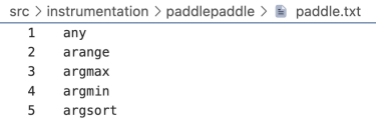
\includegraphics[width=\linewidth]{1.png}
  \caption{Work flow of Freefuzz}
\end{figure}

To extend FreeFuzz to test PaddlePaddle library, we will follow the same four steps. 
We will obtain code/models from three different sources: 1) code snippets from library documentation, 2) developer tests, and 3) DL models in the wild. 
We will then run the collected code/models with instrumentation to trace dynamic information for each covered API. 
Next, we will leverage the traced dynamic information to perform fuzz testing for each covered API. 
Finally, we will resolve the test oracle problem with differential testing and metamorphic testing.

To address the challenge of dynamic typing in Python, we will use type annotations to specify input parameter types for each API. 
By using type annotations, we can automatically determine API input parameter types and generate valid test cases.

By following the same four steps used in FreeFuzz paper and addressing challenges specific to PaddlePaddle library such as dynamic typing in Python using type annotations, 
we can extend FreeFuzz to test PaddlePaddle library and improve its quality and reliability. Additionally, we provided detailed documentation and publicly shared our code on Github (\href{https://github.com/yuehaoshi/FreeFuzz}{https://github.com/yuehaoshi/FreeFuzz}), 
which can be utilized by other researchers interested in employing the FreeFuzz methodology to test the PaddlePaddle library.
  
  \subsection{Code Collection}
  The methodology for collecting code snippets for the PaddlePaddle framework was inspired by the FreeFuzz research paper. 
  The team obtained code snippets from three primary sources, namely: (1) code snippets from the official documentation, 
  (2) testing files from the PaddlePaddle library developer tests, and (3) deep learning models in the wild. 
  The team also collected API executions of PaddlePaddle based on the same three sources.

  The official website of PaddlePaddle was the primary source of code snippets, which provided all available API names, 
  definitions, and execution examples for the latest version of the framework. To automate the process of parsing the documentation and obtaining the code snippets, 
  the team utilized the bs4 Python package. 

  The team also collected testing files from the PaddlePaddle library developer tests. 
  There are a total of 692 testing files in the latest version of PaddlePaddle, which the team obtained by cloning the latest PaddlePaddle official repository into their local machine.

  Lastly, the team obtained code from deep learning models in the wild. 
  The team collected publicly available PaddlePaddle models and utilized them as a source of real-world use cases for testing the PaddlePaddle libraries. 
  For instance, the PaddleNLP package, which is an easy-to-use and powerful NLP library that leverages PaddlePaddle as a basic structure, provided numerous Paddle API calls that were suitable for collecting APIs for fuzzing. 
  The team executed all testing files for this package to augment their API pool with this package.
    
  \subsection{instrumentation}
  

  Instrumentation is a crucial step in FreeFuzz that enables the collection of dynamic execution information for test-input generation. 
  To extend FreeFuzz to test PaddlePaddle library, we will perform code instrumentation using the same approach as used in the original paper.
  The second stage of the Freefuzz adaptation process for PaddlePaddle involves dynamic tracing with instrumentation, 
  which allows Freefuzz to intercept selected PaddlePaddle APIs and collect information about their execution, 
  including input argument values and output values. 

  Next, we will insert additional code into this representation at specific points where an API is invoked to record its dynamic information such as name, input parameters and return value.
  Once all covered APIs have been instrumented, we will run all collected code/models with instrumentation enabled. 
  During execution, whenever an instrumented API is called, its dynamic information is stored in MongoDB in JSON format to create the necessary type space, 
  API value space, and argument value space for later fuzzing stages.


  \subsection{Mutation Test}

  In this phase, We applies various mutation rules to mutate the arguments.\cite{w1}
  \newline \textbf{Mutation Rules}. The mutation rules for FreeFuzz are composed
  of two parts: type mutation and value mutation, shown in Tables 1
  and 2, respectively. Type mutation strategies include Tensor Dim
  Mutation that mutates n1-dimensional tensors to n2-dimensional
  tensors, Tensor Dtype Mutation that mutates the data types of tensors without changing their shapes, Primitive Mutation that mutates
  one primitive type into another, as well as Tuple Mutation and List
  Mutation that mutate the types of elements in collections of heterogeneous objects.\cite{w1}
  \newline Different from pytorch and tensorflow, paddle doesn't have the api to generate random complex values. Thus, the team
  created such function which is randomizing the real part and imaginary part of complex number respectively.
 
  \begin{table*}[h]
    \centering
    \caption{Type Mutation}
    \label{tab:freq}
    \begin{tabular}{ccl}
      \toprule
      Mutation Strategies&$T_1$&$T_2$\\
      \midrule
      Tensor Dim Mutation & tensor<n1,DT>& tensor<n2,DT>\\
      Tensor Dtype Mutation & tensor<n,$DT_1$>& tensor<n,$DT_2$>\\
      Primitive Mutation & $T_1$ = int|bool|float|str & $T_2$\\
      Tuple Mutation & $(T_i ^ {i\in 1...n})$&$(typemutate(T_i ^ {i\in 1...n}))$ \\
      List Mutation & $[T_i ^ {i\in 1...n}]$&$[typemutate(T_i ^ {i\in 1...n})]$ \\
    \bottomrule
  \end{tabular}
  \end{table*}

  \begin{table*}[h]
    \centering
    \caption{Value Mutation}
    \label{tab:freq}
    \begin{tabular}{ccl}
      \toprule
      Mutation Strategies&$T$&$V$\\
      \midrule
      Random Tensor Shape& tensor<n,DT>& tensor(shape=[randint()],dtype=DT)\\
      Random Tensor Value& v: tensor<n,DT>& tensor(shape=v.shape,dtype=DT).rand()\\
      Random Primitive& int|bool|float|str & rand(int|bool|float|str)\\
      Random Complex& real + imag & rand(real) + rand(imag)\\
      Random Tuple& $(T_i ^ {i\in 1...n})$&$(value\_mutate(T_i ^ {i\in 1...n}))$ \\
      Random List& $[T_i ^ {i\in 1...n}]$&$[value\_mutate(T_i ^ {i\in 1...n})]$ \\
    \bottomrule
  \end{tabular}
  \end{table*}


  We collected different types for PaddlePaddle, and decide to extend the mutation strategies used in the original paper.
  To summarize, the team has selected a subset of APIs as a proof of concept to 
  demonstrate the feasibility of applying the complete Freefuzz testing process to the PaddlePaddle package, 
  as set out in the midterm goals.

  \subsection{Test Oracle}
  The original Freefuzz paper proposed leveraging multiple execution modes during the instrumentation process to detect wrong-computation results. 
  By comparing the results obtained from different execution modes, potential DL library bugs can be detected. However, due to having only MacOS, 
  on which Paddle does not support CUDA, the team was unable to perform CUDA testing for Paddle.

  Therefore, the team focused on detecting crash bugs and performance bugs by employing mutation-based fuzzing techniques that modify existing inputs, modify data type, and generate new inputs from scratch. 
  By modifying existing inputs in various ways, FreeFuzz can identify performance issues and crash bugs that traditional unit tests may have missed.

\section{Evaluation}
  \subsection{Implementation}
  \textbf{Code Collection}. For code collected from Paddle official documentation, 
  the resulting scripts and outputs for crawling can be accessed from the $/src/reptile directory$, 
  while the API execution code snippets are available in \verb|src/reptile/code_snippets|. 
  After filtering out invalid results from the reptile tool and several API execution codes that caused instrumentation to crash, 
  the team obtained a total of 826 API names, 720 API definitions, and 1493 executable code snippets from the official PaddlePaddle documentation website.
  \par For official test source, the team cloned Paddle source code from Github and executed all \verb|test_*.py| files in Paddle/test folder using pytest as automation testing tool. 
  After removing unsupported imports by removing invalid tests, there are 2741 tests left. After executing all 2741 tests, only one more collection shown on MongoDB, 
  but the total size in database increased  \verb|2%|, indicating significant API execution overlap between official documentation code snippets and testing documents.
  For wild Paddle project source, the team collected PaddleNLP package and ran testing files inside it.

  \textbf{Instrumentation}. To implement this instrumentation stage, the team repurposed the code used for testing the PyTorch library, 
  utilizing functions such as \verb| hijack|, \verb| decorate_class|, \verb| decorate_function|, and \verb| write_fn|. Different sources of code collection require different ways of implementing instrumentation. 
  During the process, the team found that not all collected APIs are valid for instrumentation, and decided to focus on fuzzing Paddle functions, keeping 511 APIs over 720 defined APIs on the Paddle official website.
  
  \par For the code collected from the official documentation, the team executed all 1493 code snippets, but several code snippets could not compile during instrumentation due to typo errors on the Paddle official documentation examples. 
  After executing all code snippets and hijacking API execution information into MongoDB, there are a total of 420 collections in MongoDB after running all code snippets, 
  where one collection means the execution information of one API.

  \begin{figure}[h]
    \centering
    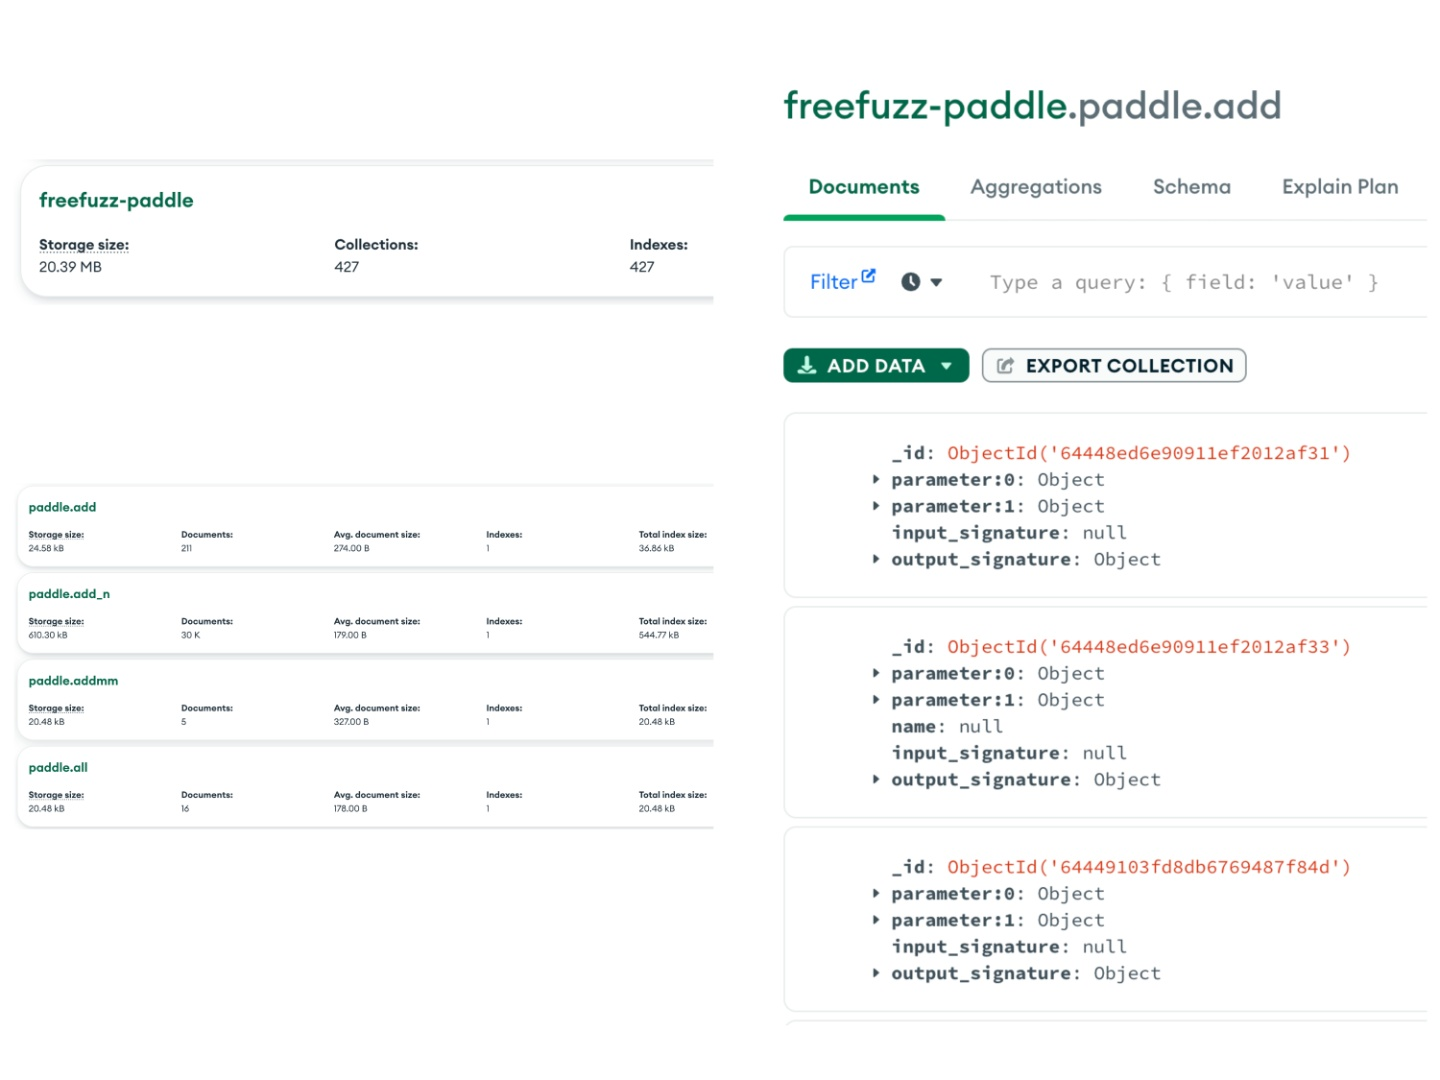
\includegraphics[width=\linewidth]{3.png}
    \caption{Database overview (left top), Database collections (left bottom), and Collection detail (right)}
  \end{figure}

  \par For the official test code, the team cloned Paddle source code from Github and executed all \verb|test_*.py| files in Paddle/test folder using pytest as automation testing tool. 
  After removing unsupported imports by removing invalid tests, there are 2741 tests left. After executing all 2741 tests, only one more collection shown on MongoDB, but the total size in database increased  \verb|2%|, 
  indicating significant API execution overlap between official documentation code snippets and testing documents.

  \par For open-source projects, the team chose the PaddleNLP package and ran testing files inside it. After executing all testing files in PaddleNLP, there are 6 more collections, and \verb|22%| more MB data increased in MongoDB, 
  meaning that PaddleNLP contributes additional API execution data in total data. PaddleNLP focuses on a specific area of APIs and generates more in-depth API calls compared to Paddle official tests, 
  which have a large proportion of unexecutable tests and false testing files that hamper their contribution to the total data.
  \newline \textbf{Mutation}.
  We use the  Mutation Algorithm proposed in \cite{w1}. The implementation details can be
  found in our project repository.
  \newline \textbf{Test Oracle}.
  Due to the lack of CUDA support on MacOS, we are unable to perform CUDA testing for Paddle.
  Since we can only run tests on CPU, we cannot do the differential testing.
  Meanwhile, the implementation of metamorphic testing is to wrap the invocation of APIs with code for timing.\cite{w1}
  
  \subsection{Metrics}
  The team will use a set of metrics to evaluate the effectiveness of Freefuzz tests for PaddlePaddle. 
  These metrics include the number of covered APIs, the size of the value space, and line coverage.
  \textbf{Number of Covered APIs.} Given the extensive range of APIs available in DL libraries, it is essential to demonstrate the total number of APIs covered as a critical indicator of the thoroughness of testing.
  
  \textbf{Size of Value Space.} Each API invocation will create a new entry in the API value space. 
  Thus, we utilize the total size of the value space for all APIs as a metric to compare and analyze different input sources. 
  In this project, we count the total amount of data size in the API value space, excluding any duplicates. 
  It is important to note that this metric is primarily used to illustrate the scale of the traced data and should not be considered as a measure of fuzzing effectiveness.
  
  \textbf{Line Coverage.} Code coverage is widely recognized as a crucial metric for evaluating the effectiveness of a test suite and its ability to provide thorough testing. 
  As part of this project, our aim was to use line coverage as a metric to assess the effectiveness of Freefuzz tests for PaddlePaddle. 
  To do this, we utilized the python coverage package during the instrumentation process. 
  Unfortunately, we encountered some issues that prevented us from obtaining reliable line coverage metrics. 
  As a result, we shifted our focus towards analyzing input source metrics and identifying failures and bugs.

  \textbf{Number of Detected Bugs.} The effectiveness of Freefuzz tests for PaddlePaddle will be evaluated by the team based on the number of bugs detected, 
  such as potential bugs, the ratio of failures to successes, and any other bugs that may be discovered during the project implementation process.

  \section{Result Analysis}
  As shown in table.\ref*{tab:freq}, we run the tests on 427 collected paddle APIs from different sources and do freefuzz tests those code.
  \begin{table*}[t]
    \centering
    \caption{FreeFuzz tests on paddle api}
    \label{tab:freq}
    \begin{tabular}{ccccc}
      \toprule
      oracle&potential bug&fail&success&time-out\\
      \midrule
      crash-oracle & 0 & 94 & 333 &0\\
      precision-oracle & 1&112&301 &13 \\
      cuda-oracle(no device supported) & 0 & 0 & 0 &0\\
    \bottomrule
  \end{tabular}
  \end{table*}


  \subsection{Input Source Study}
  The team evaluated the effectiveness of FreeFuzz for testing PaddlePaddle library by analyzing different input sources. We explored three different sources: 1) code snippets from library documentation, 2) developer tests, and 3) DL models in the wild.

  Our results showed that FreeFuzz was able to automatically trace valid dynamic information for fuzzing 427 popular APIs using each input source individually, including 420 from official documentation, 1 from official tests, and 6 from wild project such as PaddleNLP.

  As for the size of the value space, we found that the official documentation code snippets contributed the most to the total API execution data, with 80\% of the total data, followed by the wild project PaddleNLP with 18\% of the total data, and the official tests with 1.7\% of the total data.
  In summary, our Input Source Study demonstrates that FreeFuzz is effective in generating test cases for PaddlePaddle library using different input sources such as code snippets from library documentation, developer tests and DL models in the wild. 
  The proportion of API value size and API number distribution from different sources are shown in figure 3.
  \begin{figure}[h]
    \centering
    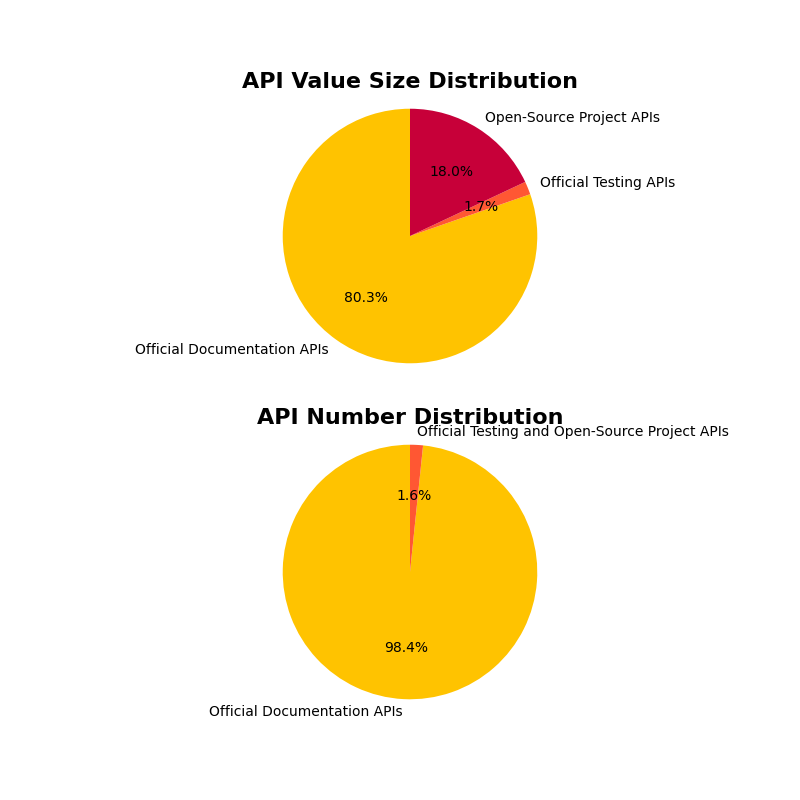
\includegraphics[width=\linewidth]{APIDist.png}
    \caption{API Value Size and API Number distribution from different sources}
  \end{figure}

  However, due to large portion of deprecated tests in official test and limited resources of large Paddle project in wild, official documentation code snippets contribute the most to the total API execution data and the other two sources are unable to contribute more APIs types,
  indicating significant API execution overlap between official documentation code snippets and testing documents.
  \subsection{Failed tests}
  Among 427 api tests, 94 tests failed. majority of them are either type error or value error. It is understandable that our mutation strategies will unavoidably generate some invalid inputs.
  \subsection{Potential bugs}
  Although we only found one potential bug as shown below, it still has value for discussion.
  Let's first take a look at the criteria for judging whether the code will produce a potential bug.
  For precision oracle, we run two tests for one specific api. According to \cite{w1}, we have this fact when 
  we run the tests on hardware M.
  \begin{equation}
    \begin{aligned}
      & precision(DT1) < precision(DT2) \Rightarrow cost(M, API_I, args, tensor \langle n, DT1 \rangle) \\
      & < cost(M, API_I, args, tensor \langle n, DT2 \rangle)
    \end{aligned}
  \end{equation}
  Thus, when time of tests on low precision datatype is 10 times longer then the time of tests on high precision datatype, we will report a potential bug. 
  In this case, low time value is 0.03082s while high time value is 0.001367s. Obviously, low time is 22.5 times longer than high time, which is larger than 10 times.
  However, due to the limitation of time, we have not found the intrinsic reason for this result. Thus, we can not confirm whether this is a real bug or not.
    
  
  \begin{lstlisting}[language=Python, numbers=left, caption={Potential bug when excuting precision oracle}, label={lst:potential_bug}]
  import paddle
  import time
  results = dict()
  arg_1_tensor = paddle.rand([1], dtype=paddle.float32)
  arg_1 = arg_1_tensor.clone()
  arg_2 = 4.0
  start = time.time()
  results["time_low"] = paddle.pow(arg_1,arg_2,)
  results["time_low"] = time.time() - start
  arg_1 = arg_1_tensor.clone().astype(paddle.float32)
  start = time.time()
  results["time_high"] = paddle.pow(arg_1,arg_2,)
  results["time_high"] = time.time() - start
\end{lstlisting}




  \subsection{Other types of errors}
  \subsubsection{paddle official documentation}
  During code collection and instrumentation part, the team collected code snippets from Paddle 2.4 version 
  official website and collected approximately 1500 code snippets. After cleaning unexecutable snippets during wrong 
  html tag of official website, there are several official code examples that would result in compile errors. After careful inspection, 
  the team found four typos on Paddle official website examples such as redundant parenthesis and illegal syntax. 
  The team then report those findings by opening several Paddle github issues as feedback\cite{r1, r2}.
  \subsubsection{paddle official test files}
  To execute all official test files, the team initially cloned the Paddle source code from Github. They attempted to execute all testing files using the CMakeList file provided in the testing folder, 
  but encountered several compile errors during the process. After conducting a thorough examination, the team discovered incompatibility issues between the CMakeList file and the current operating system. 
  Consequently, the team opted to employ pytest as an automation testing tool to execute all testing files. During the pytest process, hundreds of import errors arose due to deprecated APIs and invalid tests.

  Following the removal of unsupported imports by eliminating invalid tests, only 2741 tests remained, but a majority of them generated failure results. 
  The considerable proportion of unexecutable and failed tests impeded their contribution to the overall data. Based on the instrumentation process of the project, the team discovered several compile errors during the process. 
  After careful inspection, the team found several incompatibility issues between the CMakeList file and the current operating system.

  Therefore, the team suggests that the Paddle development team should better maintain the testing files to prevent compile errors and import errors during the testing process. 
  Additionally, they recommend providing instructions on the testing files regarding the prerequisites for executing them on various systems, if possible.
  

\section{Future Work}
In the current implementation of extending FreeFuzz to the PaddlePaddle library, several limitations exist. 
Firstly, the team has used MacOS as the testing environment, which does not support CUDA for PaddlePaddle\cite{c1}. 
Consequently, testing of CUDA related APIs in PaddlePaddle is not possible. 
To test CUDA related APIs, future developers are advised to use an operating system other than MacOS as the testing environment.

Secondly, due to limited time and resources, the team conducted the fuzzing process only a few times, 
resulting in the discovery of only one potential bug. 
To increase the probability of finding potential bugs, it is recommended that future developers run the fuzzing process multiple times.
As for the potential bug captured so far, the team targeted the reason for the bug, but failed to find the root cause, 
thus this would also be a future work to dig into.

In addition, the research team endeavored to employ the Python coverage tool in order to gauge the code coverage of the testing process. Regrettably, the team encountered unresolved difficulties pertaining to the utilization of coverage tools, which impeded the successful implementation of code coverage measurement. Notwithstanding that code coverage measurement is not the exclusive metric for assessing the efficacy of the testing process, and that an elevated code coverage does not inevitably signify a superior quality of the testing process, it remains a valuable metric for appraising and refining the testing process. Consequently, forthcoming efforts ought to be directed towards the realization of code coverage measurement for fuzzing the PaddlePaddle library.
Finally, the team only used PaddleNLP as the wild project to test FreeFuzz. 
To improve the robustness of FreeFuzz, future developers are encouraged to use multiple wild projects for testing purposes.




\begin{thebibliography}{9}
\bibitem{p1} K. He, X. Zhang, S. Ren, and J. Sun. Deep Residual Learning for Image Recognition.
In Proceedings of the IEEE Conference on Computer Vision and Pattern Recognition
(CVPR), June 2016.
\bibitem{p2} K. Simonyan and A. Zisserman. Very deep convolutional networks for large-scale
image recognition. arXiv preprint arXiv:1409.1556, 2014.
\bibitem{p3} F. A. Gers, J. Schmidhuber, and F. Cummins. Learning to forget: Continual
prediction with lstm. Neural computation, 12(10):2451–2471, 2000.
\bibitem{p4} A. Graves, A.-r. Mohamed, and G. Hinton. Speech recognition with deep recurrent
neural networks. In 2013 IEEE international conference on acoustics, speech and
signal processing, pages 6645–6649. Ieee, 2013.
\bibitem{p5} J. Chen, H. Ma, and L. Zhang. Enhanced compiler bug isolation via memoized
search. In Proceedings of the 35th IEEE/ACM International Conference on Automated
Software Engineering, pages 78–89, 2020.
\bibitem{p6} X. Li, W. Li, Y. Zhang, and L. Zhang. Deepfl: Integrating multiple fault diagnosis
dimensions for deep fault localization. In Proceedings of the 28th ACM SIGSOFT
International Symposium on Software Testing and Analysis, pages 169–180, 2019.
\bibitem{p7} Y. Yang, X. Xia, D. Lo, and J. Grundy. A survey on deep learning for software
engineering. arXiv preprint arXiv:2011.14597, 2020.
\bibitem{p8} Z. Zeng, Y. Zhang, H. Zhang, and L. Zhang. Deep just-in-time defect prediction:
how far are we? In Proceedings of the 30th ACM SIGSOFT International Symposium
on Software Testing and Analysis, pages 427–438, 2021.
\bibitem{p9} N. Akhtar and A. Mian. Threat of adversarial attacks on deep learning in computer
vision: A survey. Ieee Access, 6:14410–14430, 2018.
\bibitem{p10} N. Carlini, A. Athalye, N. Papernot, W. Brendel, J. Rauber, D. Tsipras, I. Goodfellow,
A. Madry, and A. Kurakin. On evaluating adversarial robustness. arXiv preprint
arXiv:1902.06705, 2019
\bibitem{p11} I. J. Goodfellow, J. Shlens, and C. Szegedy. Explaining and harnessing adversarial
examples. arXiv preprint arXiv:1412.6572, 2014.
\bibitem{p12} F. Harel-Canada, L. Wang, M. A. Gulzar, Q. Gu, and M. Kim. Is neuron coverage a
meaningful measure for testing deep neural networks? In Proceedings of the 28th
ACM Joint Meeting on European Software Engineering Conference and Symposium
on the Foundations of Software Engineering, pages 851–862, 2020.
\bibitem{p13} J. Kim, R. Feldt, and S. Yoo. Guiding deep learning system testing using surprise
adequacy. In 2019 IEEE/ACM 41st International Conference on Software Engineering
(ICSE), pages 1039–1049. IEEE, 2019.
\bibitem{p14} L. Ma, F. Juefei-Xu, F. Zhang, J. Sun, M. Xue, B. Li, C. Chen, T. Su, L. Li, Y. Liu,
et al. Deepgauge: Multi-granularity testing criteria for deep learning systems. In
Proceedings of the 33rd ACM/IEEE International Conference on Automated Software
Engineering, pages 120–131, 2018.
\bibitem{p15} Y. Tian, K. Pei, S. Jana, and B. Ray. Deeptest: Automated testing of deep-neuralnetwork-driven autonomous cars. In Proceedings of the 40th international conference on software engineering, pages 303–314, 2018.
\bibitem{p16} M. Zhang, Y. Zhang, L. Zhang, C. Liu, and S. Khurshid. Deeproad: Gan-based
metamorphic testing and input validation framework for autonomous driving
systems. In 2018 33rd IEEE/ACM International Conference on Automated Software
Engineering (ASE), pages 132–142. IEEE, 2018.
\bibitem{p17} H. Zhou, W. Li, Z. Kong, J. Guo, Y. Zhang, B. Yu, L. Zhang, and C. Liu. Deepbillboard: Systematic physical-world testing of autonomous driving systems. In 2020
IEEE/ACM 42nd International Conference on Software Engineering (ICSE), pages
347–358. IEEE, 2020.
\bibitem{p18} H. V. Pham, T. Lutellier, W. Qi, and L. Tan. CRADLE: Cross-Backend Validation
to Detect and Localize Bugs in Deep Learning Libraries. In 2019 IEEE/ACM 41st
International Conference on Software Engineering (ICSE), pages 1027–1038, 2019.
\bibitem{p19} Z. Wang, M. Yan, J. Chen, S. Liu, and D. Zhang. Deep learning library testing
via effective model generation. In Proceedings of the 28th ACM Joint Meeting on
European Software Engineering Conference and Symposium on the Foundations of
Software Engineering, pages 788–799, 2020.
\bibitem{p20} Ma, Y., Yu, D., Wu, T. and Wang, H., 2019. PaddlePaddle: An open-source deep learning platform from industrial practice. Frontiers of Data and Domputing, 1(1), pp.105-115.

\bibitem{w1} Wei, A., Deng, Y., Yang, C.,  Zhang, L. (2022, May). Free lunch for testing: Fuzzing deep-learning libraries from open source. In Proceedings of the 44th International Conference on Software Engineering (pp. 995-1007).
\bibitem{c1} PaddlePaddle. \textit{Installation Guide}. PaddlePaddle. Accessed May 4, 2023. \url{https://www.paddlepaddle.org.cn/documentation/docs/en/install/index_en.html}.
\bibitem{r1} PaddlePaddle, GitHub. Issue 53437, https://github.com/PaddlePaddle/Paddle/issues/53437, Accessed May 4, 2023.
\bibitem{r2} PaddlePaddle, GitHub. Issue 53437, https://github.com/PaddlePaddle/Paddle/issues/53438, Accessed May 4, 2023.

\end{thebibliography}
\end{document} 
\endinput
%%
%% End of file `sample-sigconf.tex'.
